% ----
% COMP1204 CW1 Report Document
% ----
\documentclass[]{article}

% Reduce the margin size, as they're quite big by default
\usepackage[margin=1in]{geometry}

%Fix double quotes
\usepackage[T1]{fontenc}
\usepackage{textcomp}

% Colour the code
\usepackage{listings}
\usepackage{xcolor}
\usepackage{graphicx}

\definecolor{blue}{rgb}{0,0,0.9}
\definecolor{red}{rgb}{0.9,0,0}
\definecolor{purple}{rgb}{0.58,0,0.82}
\definecolor{background}{rgb}{0.97,0.97,0.93}

\lstdefinestyle{bash_style}{
    commentstyle=\color{blue},
    keywordstyle=\color{purple},
    stringstyle=\color{red},
    backgroundcolor=\color{background},
    showspaces=false,
    showstringspaces=false,
    captionpos=b
}
\lstset{language=bash,style=bash_style,breaklines}

\title{COMP1204: Data Management \\ Coursework One: Hurricane Monitoring }
\author{Andrew Milne \\ am4n23}

% Actually start the report content
\begin{document}
\lstset{upquote=true}

% Add title, author and date info
\maketitle

\section{Introduction}

This report aims to extract and analyse data regarding a variety of tropical storms from KML files produced by the National Hurricane Center. It will accomplish this through a Unix bash script, which will create a CSV file containing the desired information of a single storm. This can either be read manually or be input to an existing Unix bash script, which creates a map of the storm's location over time based on the data input.

The information extracted by the CSV script is the following:

\begin{itemize}
    \item Timestamp, in the format [HHMM] UTC [MONTH] [DATE], e.g. 1200 UTC JAN 01
    \item Latitude, with the direction specified, e.g. 12.5 N
    \item Longitude, with the direction specified, e.g. -37.5 W
    \item Minimum Pressure at Sea Level, in millibars, e.g. 1000 mb
    \item Maximum Intensity, in knots, e.g. 40 knots
\end{itemize}

\section{Create CSV Script}

\begin{lstlisting}[caption=Script to create a CSV file using an input KML file]
#!/bin/bash

#Set up input and output paths as variables
kml_input_path=$1
csv_output_path=$2

echo "Converting "${kml_input_path}" -> "${csv_output_path}"..."

#Create CSV file from the input using awk
awk -F '[<>]' 'BEGIN{string=""} #Start by designating < and > as delimiters, allowing us to search by command, and create a string to put information in
{if($2=="/Placemark"){print string; string=""}} #If we reach a /Placemark command, this is the end of a piece of data, so we can print and reset the string to prepare it for the next piece of information
{if($2=="lat"){ #lat = latitude command
    string = string $3; #$3 contains the data, so we append it to the string
    if(($3+0)<0){string = string " S,"} #Append south and delimiter if negative number
    else{string = string " N,"} #Append north and delimiter if positive number
}}
{if($2=="lon"){ #lon = longitude command
    string = string $3; #Append data
    if(($3+0)<0){string = string " W,"} #Append west and delimiter if negative number
    else{string = string " E,"} #Append east and delimiter if positive number
}}
{if($2=="intensity"){ #intensity = intensity command
    string = string $3; #Append data
    string = string " knots," #Append unit and delimiter
}}
{if($2=="minSeaLevelPres"){ #minSeaLevelPres = minimum sea level pressure command
    string = string $3; #Append data
    string = string " mb," #Append unit and delimiter
}}
{if($2=="dtg"){
    string = string $3; #Append data
    string = string ","; #Append delimiter
}}' ${kml_input_path} | sed "s/\n//g" | sed "s/)/\n/g" | awk -F '[,]' 'BEGIN{print "Timestamp,Latitude,Longitude,MinSeaLevelPressure,MaxIntensity"} #We now have a csv file, but we need to put the columns in the correct order.
{string="";
string = string $5;
string = string ",";
string = string $1;
string = string ",";
string = string $2;
string = string ",";
string = string $4;
string = string ",";
string = string $3;
print string}' > ${csv_output_path} #And finally, put the result into the output.

echo "Done!"
\end{lstlisting}

\newpage

\section{Storm Plots}

\begin{figure}[h!]
    \centering
    \begin{minipage}{0.5\linewidth}
        \centering
        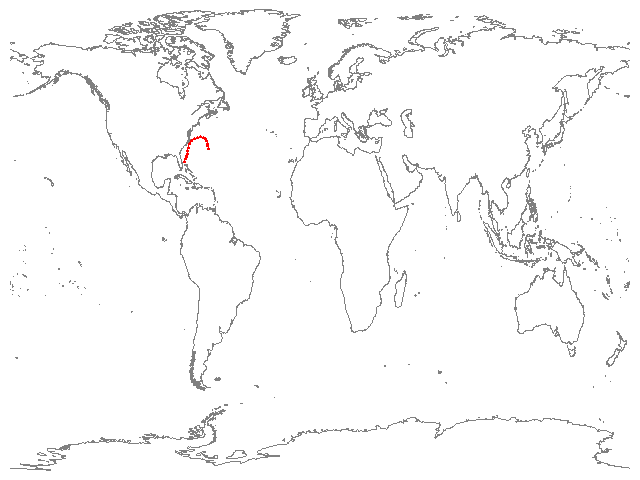
\includegraphics[width=0.9\textwidth]{al_2020_01.png}
        \caption{Storm corresponding to al012020.kml.}
    \end{minipage}\hfill
    \begin{minipage}{0.5\linewidth}
        \centering
        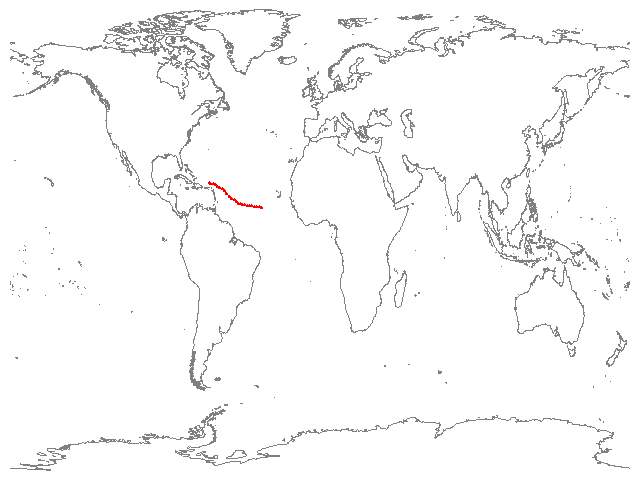
\includegraphics[width=0.9\linewidth]{al_2020_11.png}
        \caption{Storm corresponding to al112020.kml.}
    \end{minipage}
\end{figure}

\begin{figure}[h!]
    \centering
    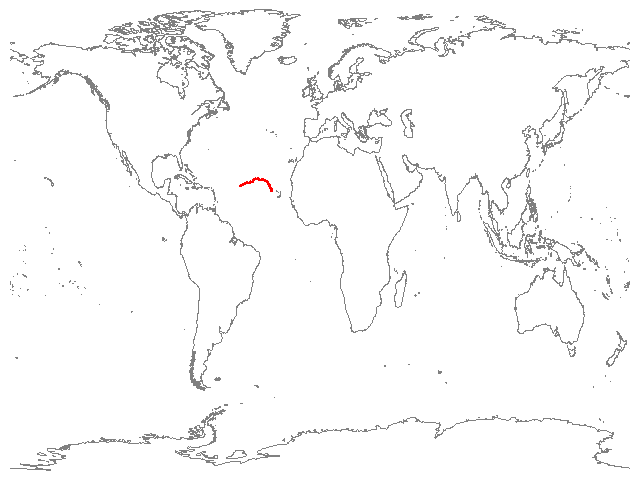
\includegraphics[width=0.45\linewidth]{al_2020_21.png}
    \caption{Storm corresponding to al212020.kml.}
\end{figure}

\section{Git usage}

After starting the merge using \lstinline{git merge python-addon}, I was made aware of a merge conflict in \lstinline{python-plot-script.py}. As a result, I used \lstinline{vim python-plot-script.py} to access the code and determine the correct alterations to make. These comprised the following:

\begin{enumerate}
    \item Some of the imports were in a different order between branches, and the \lstinline{main} branch also had \lstinline{math} imported. I initially used the \lstinline{main} branch for this due to the extra import, though later removed the \lstinline{math} import as it was not used within either branch.
    \item The user key differed between branches, and the \lstinline{python-addon} branch formatted this differently ("\lstinline{user_key= }" rather than "\lstinline{user_key = }"). I used the \lstinline{python-addon} branch for this, but changed it to the formatting used in the \lstinline{main} branch.
    \item The \lstinline{python-addon} branch had a spelling mistake ("fr" instead of "for"), so I used the \lstinline{main} branch for that section as it was the only difference.
    \item The \lstinline{python-addon} branch had an additional \lstinline{plot_all_csv_intensity} function, identical to main's \lstinline{plot_all_csv_pressure} function except replacing "pressure" with "intensity". I kept this addition.
    \item The notations designating merge conflicts were removed, as these had now all been resolved.
    \item The \lstinline{python-addon} branch was deleted and the new file was committed.
\end{enumerate}

As such, the final version of \lstinline{python-plot-script.py} is:

\begin{lstlisting}[caption=The final version of python-plot-script.py after all conflicts were resolved.]
import pandas as pd
import matplotlib.pyplot as plt
import os
import glob
user_key = 26917

def plot_all_csv_pressure():
    path = os.getcwd()
    csv_files = glob.glob(os.path.join(path, '*.csv')) 

    for f in csv_files:
        storm = pd.read_csv(f)
        storm['Pressure'].plot()
        plt.show()
		
def plot_all_csv_intensity():
    path = os.getcwd()
    csv_files = glob.glob(os.path.join(path, '*.csv'))
    
    for f in csv_files:
        storm = pd.read_csv(f)
        storm['Intensity'].plot()
        plt.show()
\end{lstlisting}

\end{document}